%%% Copyright (C) 2020 Vincent Goulet
%%%
%%% Ce fichier fait partie du projet
%%% «Rédaction avec LaTeX»
%%% https://gitlab.com/vigou3/formation-latex-ul
%%%
%%% Cette création est mise à disposition sous licence
%%% Attribution-Partage dans les mêmes conditions 4.0
%%% International de Creative Commons.
%%% https://creativecommons.org/licenses/by-sa/4.0/

%% Normes de présentation visuelle 2018
%%
%% - grille de 8 unités de haut
%% - 1 mesure = 1/8 d'unité
%% - bande identitaire de 1 mesure placée au bas de la 7e unité
%% - logo haut de 4 mesures avec blancs de deux mesures en haut et
%%   en bas
%% - blanc équivalent à la largeur du blason à droite du logo
%% - bande or de la largeur du logo + blanc à droite
%%
%% Dimensions du logo UL
%%
%% hauteur: 128
%% largeur totale: 310
%% largeur blason: 100
%% valeur clé: (310 + 100)/128 = 3.2031125
%%
%% Dimensions de l'image
%%
%% hauteur: 55 mesures - 1pt (filet) = 54.9191919 mesures
%% largeur: 160mm
%% ratio largeur/hauteur: 160/77.23

\begingroup
\TPGrid{16}{64}
\textblockorigin{0mm}{0mm}
\setlength{\parindent}{0mm}
\setlength{\imageheight}{54.9191919\TPVertModule}
\setlength{\logoheight}{4\TPVertModule}
\setlength{\bandeorwidth}{3.203125\logoheight}
\setlength{\banderougewidth}{\paperwidth}
\addtolength{\banderougewidth}{-\bandeorwidth}
\setlength{\bandeorheight}{\TPVertModule}
\setlength{\banderougeheight}{\TPVertModule}
\setlength{\textwidth}{\paperwidth}
\addtolength{\textwidth}{-2\TPHorizModule}

\def\titlefmt{%
  \titlefontOS\bfseries\fontsize{24}{24}\selectfont%
  Rédaction avec
  \lucida\mdseries%
  {\textbackslash}title%
  \raisebox{-6pt}{\fontsize{48}{48}\selectfont%
    \{%
    \fontsize{40}{40}\selectfont%
    \LaTeX
    \fontsize{48}{48}\selectfont%
    \}\par}}
\def\subtitlefmt{%
  \titlefontOS\bfseries\fontsize{10}{11}\selectfont%
  Premiers pas\par}
\def\authorfmt{%
  \titlefontOS\bfseries\fontsize{14}{14}\selectfont%
  Vincent Goulet\par}
\def\affiliation{%
  \titlefontOS\mdseries\fontsize{10}{11}\selectfont%
  Professeur titulaire \\
  École d'actuariat, Université Laval}
\def\edition{%
  \titlefontOS\mdseries\fontsize{10}{11}\selectfont%
  Édition {\titlefontFC\year}.\month}

%%%
%%% Page de titre
%%%

\begin{frame}[plain]
  %% bandeau identitaire
  \begin{textblock*}{\paperwidth}[0,1](0mm,56\TPVertModule)
    \textcolor{rouge}{\rule{\banderougewidth}{\banderougeheight}}% % bande rouge
    \textcolor{or}{\rule{\bandeorwidth}{\bandeorheight}}           % bande or
  \end{textblock*}

  %% logo UL
  \begin{textblock*}{\bandeorwidth}(\banderougewidth,58\TPVertModule)
    
\includegraphics[height=\logoheight,keepaspectratio=true]{ul_p}
  \end{textblock*}

  %% image de fond
  \begin{textblock*}{\paperwidth}(0mm,0mm)
    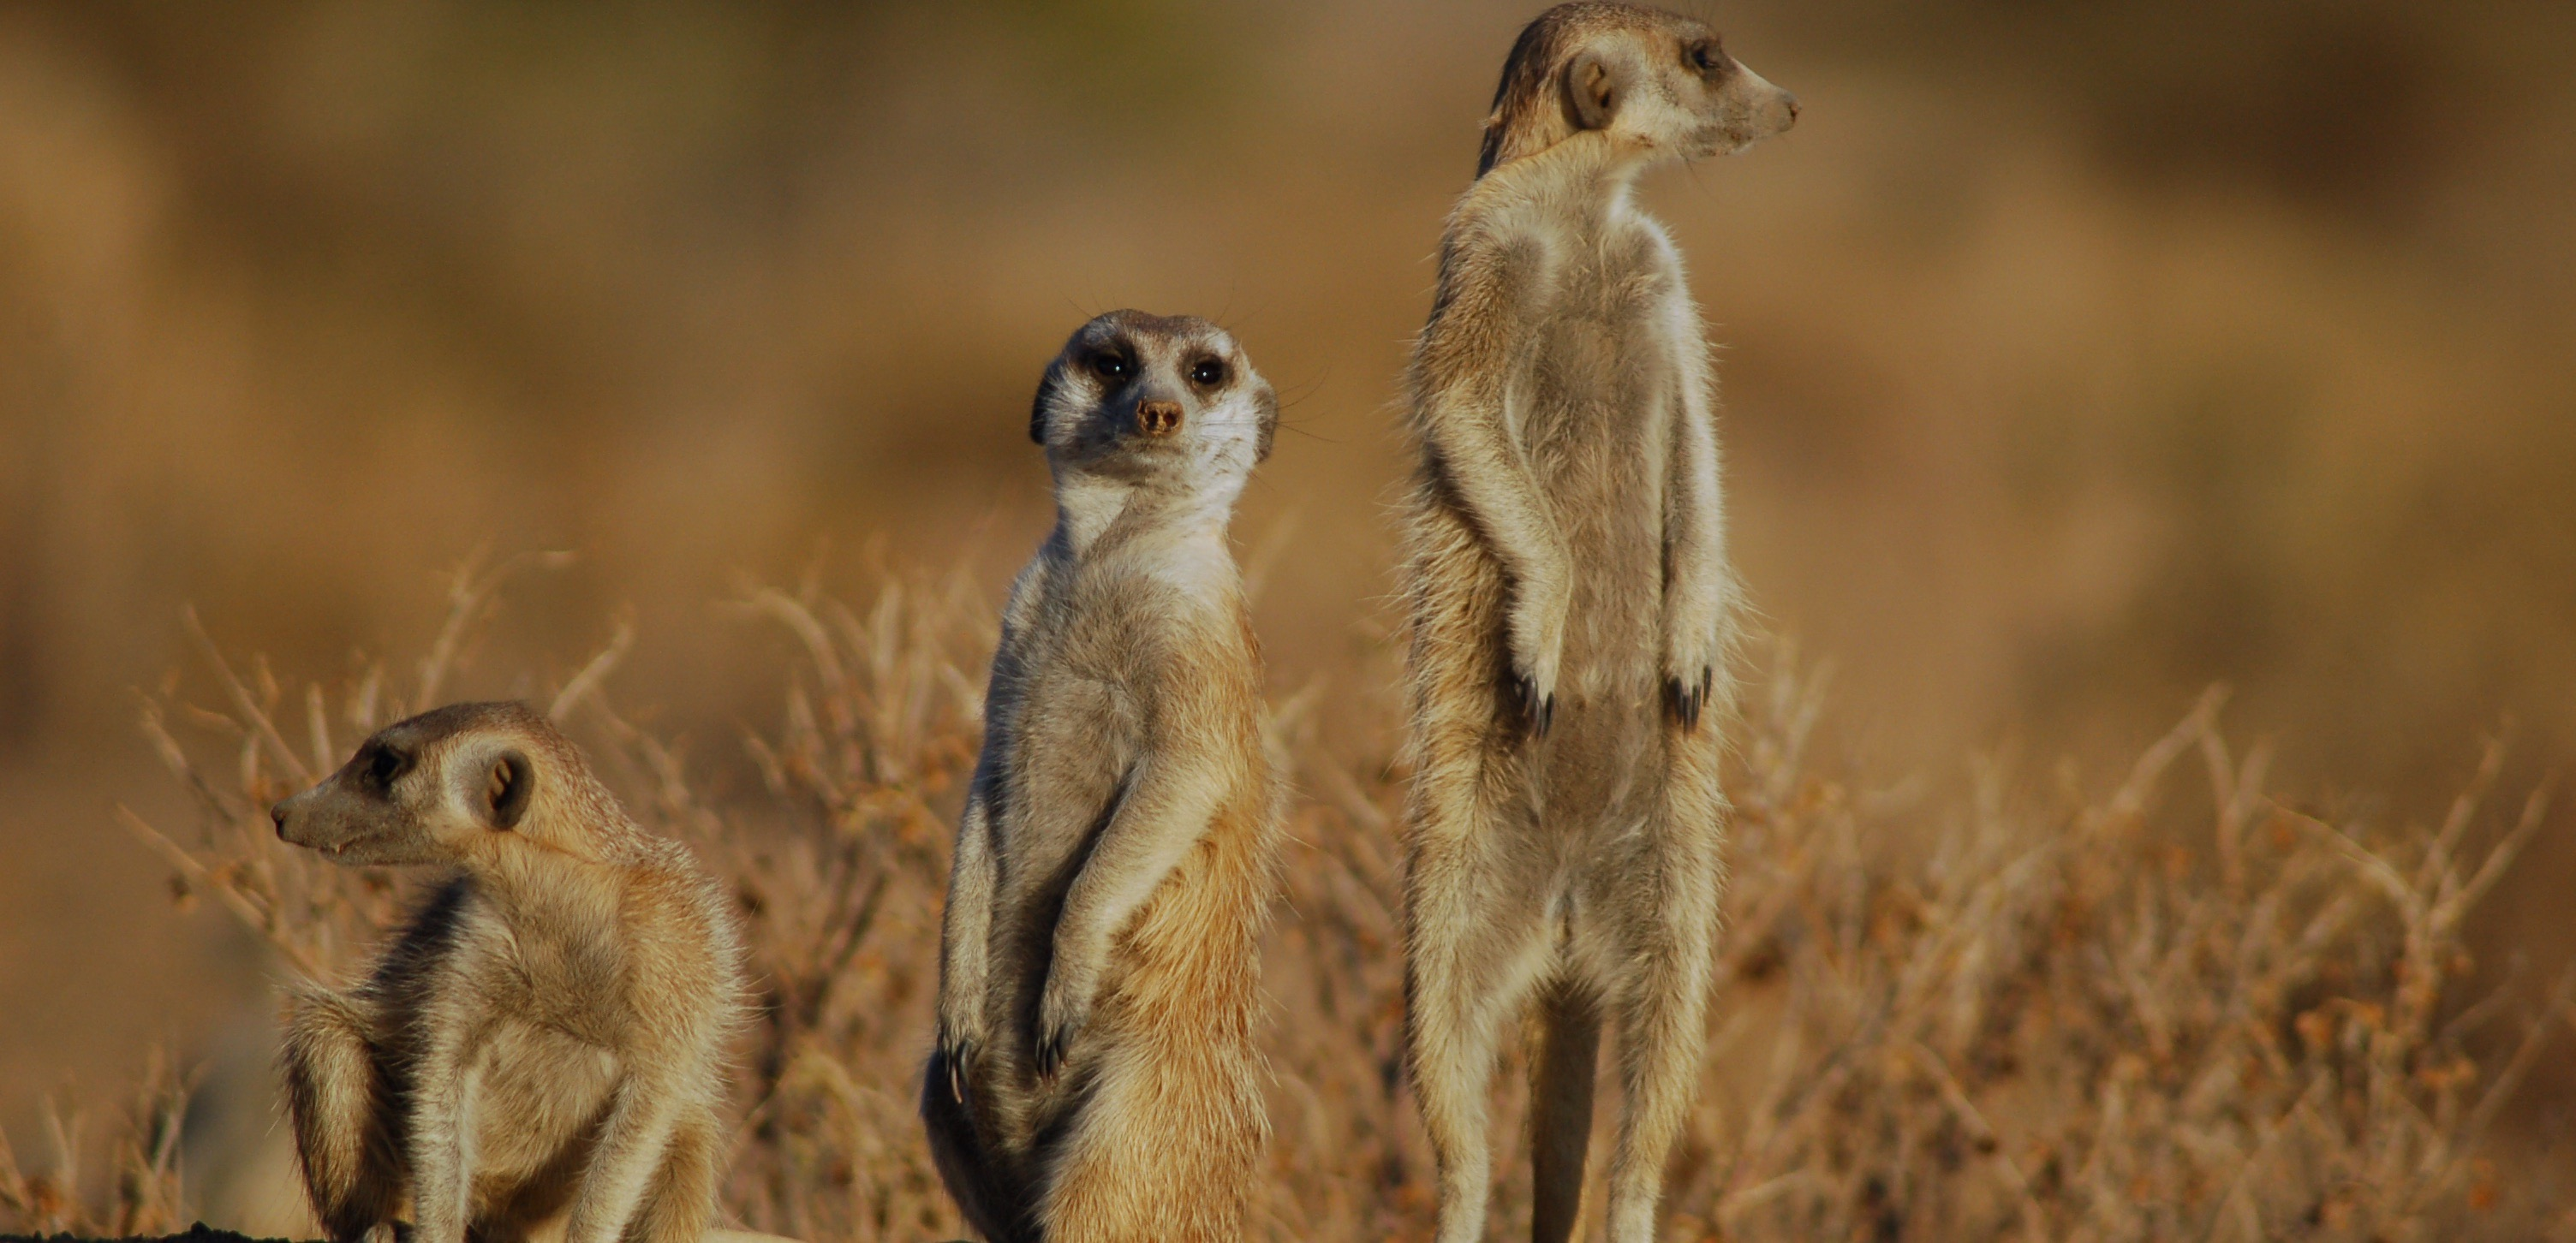
\includegraphics[height=\imageheight,width=\paperwidth]{images/Suricates_Namibia-2-diapos}
  \end{textblock*}

  %% titre
  \begin{textblock*}{\banderougewidth}(0.8\TPHorizModule,4\TPVertModule)
    \textcolor{black!10}{\titlefmt}
  \end{textblock*}

  %% sous-titre (premiers pas)
  \begin{textblock*}{\banderougewidth}(0.8\TPHorizModule,13\TPVertModule)
    \textcolor{black!10}{\subtitlefmt}
  \end{textblock*}
\end{frame}

%%%
%%% Page frontispice
%%%

\begin{frame}[plain]
  %% titre
  \begin{textblock*}{\banderougewidth}(0.8\TPHorizModule,4\TPVertModule)
    \titlefmt
  \end{textblock*}

  %% sous-titre
  \begin{textblock*}{\banderougewidth}(0.8\TPHorizModule,13\TPVertModule)
    \subtitlefmt
  \end{textblock*}

  %% auteur
  \begin{textblock*}{\textwidth}(0.8\TPHorizModule,28\TPVertModule)
    \authorfmt
  \end{textblock*}

  %% affiliation
  \begin{textblock*}{\textwidth}(0.8\TPHorizModule,33\TPVertModule)
    \affiliation
  \end{textblock*}

  %% édition
  \begin{textblock*}{\textwidth}(0.8\TPHorizModule,58\TPVertModule)
    \edition
  \end{textblock*}
\end{frame}
\endgroup

%%% Local Variables:
%%% TeX-master: "formation-latex-ul-diapos"
%%% TeX-engine: xetex
%%% coding: utf-8
%%% End:
